\section{Diverse Temporal Planning}
\label{background: Diverse Temporal}

Our approach to diverse temporal planning builds upon the top-$k$ approach in \cite{katz2019reshaping} using a {\em plan forbidding reformulation} as in \cite{katz2018novel} . 

The top-$k$ approach defines metrics in order to measure how close plans are to the best subset of all known plans, while the forbidding reformulation constitutes a diverse planning algorithm that instead of modifying the planner, in order to find a dissimilar solution, modifies the planning task itself. The reformulation occurs after each iteration (during which a new plan is found) and alters the planning task in such a way as to forbid the possibility of finding the same solution that was obtained in the previous iteration.
%%

The main challenge we address here is that temporal plans are not a sequence of instantaneous happenings (IHs), but rather a schedule, and thus the top-$k$ approach does not apply directly. Therefore, we first define the {\em temporal plan skeleton} of a solution to a temporal planning task.

\begin{definition}[\textbf{Temporal Plan Skeleton}]
Given a planning task $\Pi = \langle F,A,I,G \rangle$ and a solution $\tau$. 
The temporal plan skeleton (TPS) $\pi$ is the sequence of the IHs in $\tau$ (without their time stamps).
\end{definition}

In other words, by observing only the sequence of occurrences in a temporal planning schedule, i.e. \textit{action-start} and \textit{action-end} events, we can refer to this TPS as a sequential plan for our diverse planning purposes. \\
We now define the \textit{TPS suffix} which will come in handy in section \ref{generating: merging} when choosing time-points for merging.

\begin{definition}[\textbf{TPS Suffix}]
Given a TPS $\pi$ and an IH $a \in \pi$. The TPS suffix of $\pi$ from $a$, denoted $\Sigma^\pi_a$, is the ordered sequence of IHs in $\pi$ from right after $a$ occurs (excluding $a$) until the end of the TPS.
\end{definition}


The objective of diverse temporal planning is to find dissimilar solutions to the temporal planning task $\Pi$. We argue that two different plans, with the same TPS, and which vary only in their time stamps, are not very different. Specifically, for the purposes of merging these plans into a TPN, they are not different at all, as the TPN executive will make the scheduling decisions. Thus, we define two plans to be different if and only if they have a different TPSs.

The diverse top-$k$ planning approach \cite{katz2019reshaping} works iteratively by calling a planner to obtain a solution $\tau$, then creating a modified planning task which eliminates the solution $\tau$, calling the planner again, and so forth.
Thus, to apply this approach to temporal planning, we create a {\em temporal plan elimination formulation}, which takes as input a temporal planning task $\Pi$ and a solution $\tau$, and creates a modified temporal planning task $\Pi'$ which eliminates all solutions which share the same TPS as $\tau$ (while all other solutions remain valid).

The main technical challenge here is that temporal planning is performed with durative actions, while the {\em plan forbidding reformulation} \cite{katz2018novel} works on IHs (as in classical planning). Furthermore, the plan forbidding reformulation is based on detecting when the current candidate plan deviates from the plan to forbid, which is simpler for classical planning. 

To overcome this challenge, we think of each durative action $a$ as two IHs; $a_{\vdash}$ at the start and $a_{\dashv}$ at the end. Note that a TPS is determined by the order of the IHs, similarly to a classical plan. 
Thus, if we could somehow plan with IHs (while still respecting action durations, invariant conditions, and temporal constraints) we could use the classical planning approach directly.
While this is not possible, we can think of a durative action as a pair of two IHs, and look at five different points where a durative action might deviate from the given TPS $\pi$. These are illustrated in Figure \ref{fig:compilation}, and correspond to the five cases described below.

\begin{figure}
\centering
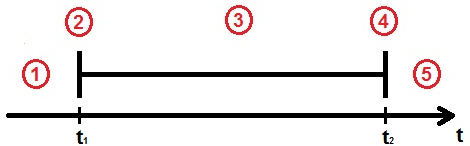
\includegraphics[width=0.6\textwidth]{graphics/compilation.jpg}
\caption{All the possible points to deviate from TPS $\pi$, from the point of view of the $i^{th}$ action in $\pi$, $a_i$.} \label{fig:compilation}
\end{figure}

\begin{description}
\item[\textbf{Case 1:}] We have already deviated from $\pi$ before $a$ started. 
\item[\textbf{Case 2:}] We followed $\pi$ until now, but action $a$ is different than the $i^{th}$ action in $\pi$.
\item[\textbf{Case 3:}] Action $a$ starts according to $\pi$, but between $a_{\vdash}$ and  $a_{\dashv}$, another instantaneous event occurs, which deviates from $\pi$.
\item[\textbf{Case 4:}] Action $a$ starts according to $\pi$, but the end event $a_{\dashv}$ is not according to $\pi$, i.e., the end event is not according to the sequence. This occurs when some other event should have occurred before $a_{\dashv}$.
\item[\textbf{Case 5:}] Action $a$ starts and ends according to $\pi$. This case is when $\pi$ is being followed, and a future action will deviate.
\end{description}

Having described these 5 cases, we can now describe our {\em temporal plan elimination formulation}. This formulation has 6 different versions of each durative action that takes part in the plan: one for each of the above five cases, and one for actions which do not appear in $\pi$. Also, similarly to the top-$k$ approach \cite{katz2018novel}, we introduce new proposition to encode deviation from $\pi$. Specifically, for a given TPS with $n$ IHs, we use $2n+2$ propositions: $2n+1$ to encode the sequence $\pi$, and another for representing whether we have already deviated. Note, that only durative action participating in the plan to forbid will be multiplied, and not the entire space of durative actions.

We now formally describe our formulation. Let $\Pi = \langle F,A,I,G \rangle$ be a planning task, and $\tau = \langle a_1, t_1, d_1\rangle ,...,\langle a_n, t_n, d_n\rangle$ be some temporal plan with a corresponding TPS $\pi$, where $i$ and $i'$ are the time indexes of $a_{\vdash}$ and $a_{\dashv}$ appropriately in $\pi$. The planning task $\Pi' = \langle F', A', I', G'\rangle$ is defined as follows:
% \begin{figure}[h]
% \centering
% \includegraphics[width=0.5\textwidth]{formulation.png}
% \end{figure}

\begin{itemize}
\item $F' = F \cup \{ p, p_0,..., p_{2n}\}$,
\item $A' = \{a^0 \ |\ a \in A, a \not\in \tau \} \cup  \{a^1,a^2,a^3,a^4,a^5 \ |\ a \in \tau \}$  \\
where:
\begin{align*}
a^0 = & \langle \text{pre}_{\vdash}(a), \text{eff}_{\vdash}(a) \cup \{p\} ,\text{inv}(a), \text{pre}_{\dashv}(a), \text{eff}_{\dashv}(a)\rangle\\ 
%
a^1 = & \langle \text{pre}_{\vdash}(a) \cup \{p\} , \text{eff}_{\vdash}(a), \text{inv}(a), \text{pre}_{\dashv}(a), \text{eff}_{\dashv}(a)\rangle\\
%
a^2 = & \langle \text{pre}_{\vdash}(a) \cup \{\neg p, \neg p_{i-1}\}, \text{eff}_{\vdash}(a) \land p, \text{inv}(a), 
 \text{pre}_{\dashv}(a),\text{eff}_{\dashv}(a)\rangle\\
%
a^3 = & \langle \text{pre}_{\vdash}(a) \cup \{\neg p, p_{i-1}\}, \text{eff}_{\vdash}(a) \land \neg p_{i-1} \land p_i, \text{inv}(a), \text{pre}_{\dashv}(a) \cup \{p\}, \text{eff}_{\dashv}(a)\rangle \\
%
a^4 =  & \langle \text{pre}_{\vdash}(a) \cup \{\neg p, p_{i-1}\}, \text{eff}_{\vdash}(a) \land p_{i-1} \land p_i, \text{inv}(a), \text{pre}_{\dashv}(a) \cup \{\neg p, \neg p_{i'-1}\}, \\ 
& \text{eff}_{\dashv}(a) \land p \rangle \\
%
a^5 = & \langle \text{pre}_{\vdash}(a) \cup \{\neg p, p_{i-1}\}, \text{eff}_{\vdash}(a) \land \neg p_{i-1} \land p_i, \text{inv}(a), \text{pre}_{\dashv}(a) \cup \{\neg p, p_{i'-1}\}, \\
&\text{eff}_{\dashv}(a) \land \neg p_{i'-1} \land p_{i'} \rangle
\end{align*}
\item $I' = I \cup \{p_0\}$
\item $G' = G \cup \{p\}$
\end{itemize}

\paragraph{Explaining the reformulation} For ease of presentation, we abuse notation and say that a temporal action $a$ is along $\pi$, when $a_{\vdash},a_{\dashv} \in \pi$ with indexes $i, i'$.
The variable $p$ represents a deviation from $\pi$, so it starts as false, and becomes true when the sequence of actions applied is not a prefix of $\pi$. Once the value $p$ is achieved, it remains true. $p$ is also part of the new goal, $G'$, as the objective here is to find a deviation from $\pi$.

Propositions $p_0, ..., p_{2n}$ encode the progress along the TPS $\pi$, before deviating from it. 
Actions $a^0$ are the activities that do not appear in $\pi$, thus automatically indicate deviation from $\pi$ and achieve $p$.
The actions $a^1, ..., a^4$ are copies of actions in $\pi$, 
corresponding to cases $1...4$ above. 
%for the cases when $\pi$ is already been discarded from consideration, and  $\bar p$ has been achieved, according to the cases described before. 
$a^5$ are copies of actions along $\pi$, these actions are responsible for following the sequence $\pi$ and are applicable only while the sequence is still followed, i.e. $p$ is false. Note that in all five cases when an action along $\pi$ has more than one instance, each instance is treated as a different action with a different corresponding $p_i$ variable indicating its position in the sequence. The convention in the reformulation is that the preconditions are sets which requirements are added to, and effects are sets comprised of delete and add effects, thus the conjunction between delete and add effects of the auxiliary variables.
% \footnote{The following theorem and an example will be made available during rebuttal if requested (as per the FAQ), and will be available in the final version of the paper with extra pages purchased.}

\begin{theorem}
Let $\Pi$ be a temporal planning task and $\tau$ a solution with TPS $\pi$. The task $\Pi'$ is a plan elimination reformulation of $\Pi$ and $\pi$.
\end{theorem}
Running the plan elimination reformulation on our input temporal planning task iteratively will yield the diverse solutions we desire.
